Ein Problem der Hopfield-Netze ist, dass sie sich häufig in einem lokalen Minimum stabilisieren statt im angestrebten globalen Minimum.
Abhilfe davon schaffen sogenannte statistische Methoden, bei denen die Neuronen ihren Zustand nicht mehr \emph{deterministisch}, sondern \emph{zufällig} nach einer Wahrscheinlichkeitsverteilung ändern.

Die \emph{Boltzmann-Maschine} ist eine solche Methode. Es handelt sich um einen \emph{unüberwachten} Lernalgorithmus, welcher die gleiche rekurrente Netzstruktur wie Hopfield-Netze verwendet. Boltzmann-Maschinen unterscheiden sich jedoch durch eine andere (stochastische) Aktivierungsfunktion und durch ein anderes Lernverfahren.



% ------------------------------------------------------------------------
% ------------------------------------------------------------------------
\section*{Lernverfahren}
Das Lernverfahren der Boltzmann-Maschine hat Ähnlichkeit mit dem technischen Verfahren zum Ausglühen eines Metalls: Zuerst wird das Metall über den Schmelzpunkt erhitzt, danach erfolgt ein langsames Abkühlen (vgl. Abschnitt zu \emph{simulated annealing}).

Bei hohen Temperaturen besitzen die Metallatome \emph{hohe Energien} und können sich nahezu frei bewegen. Dabei werden zufällig alle möglichen Konfigurationen eingenommen. Beim langsamen Abkühlen verringern sich die Energien und das System stabilisiert sich schließlich in einem \emph{Zustand mit minimaler Energie} (globales Minimum der Energiefunktion).
Bei gegebener Temperatur ist die Wahrscheinlichkeitsverteilung der Energie des Systems durch den Boltzmann-Faktor
\[
	e^{(\frac{-E}{kT})}	
\]
gegeben. Dabei sind $E$ die Energie des Systems, $k$ die Boltzmann-Konstante und $T$ die absolute Temperatur.
Für hohe Temperaturen $T$ hat das System eine hohe Wahrscheinlichkeit, hohe Energie zu besitzen. Bei niedrigen Temperaturen $T$ gibt es eine endliche, wenn auch geringe Wahrscheinlichkeit, dass das System trotzdem eine hohe Energie besitzt.


% ------------------------------------------------------------------------
\subsection*{Energie und Aktivierungsfunktion}
Die Energie einer Boltzmann-Maschine wird in gleicher Weise wie bei einem Hopfield-Netz durch die Summe aller paarweisen Energien der Neuronen definiert, üblicherweise nach der Formel
\[
	E = - \sum_{i < j} w_{ij} \cdot o_i \cdot o_j + 
		\sum_i \theta_j \cdot o_j
\]
wobei wie üblich $w_{ij}$ die Verbindung zwischen Neuron $i$ und Neuron $j$, $o_i$ die Ausgabe von Neuron $i$ (entweder 0 oder 1) und $\theta_i$ der Schwellenwert von Neuron $i$ ist.
Aktivierung und Ausgabe einer Zelle sind in diesem Modell identisch, es gilt also $a_j = o_j$.
Man beachte, dass die Summation über alle $i$, $j$ mit $i < j$, d.h. nur über die eine Hälfte der Gewichtsmatrix erfolgt, da die andere \emph{symmetrisch} dazu ist.

Wie bei binären Hopfield-Netzen ist die Energiedifferenz, die durch das Umschalten der Ausgabe eines einzelnen Neurons $k$ entsteht, gegeben durch
\[
	\Delta E_k = net_k - \theta_k = \sum_i (w_{ik} \cdot o_i - \theta_k)
\]

Mit dem \emph{Trick} des "`on"'-Neurons lassen sich die beiden Formeln wie folgt verkürzen:
\begin{align*}
	E &= \sum_{i < j} w_{ij} \cdot o_i \cdot o_j \\
	\Delta E_k &= net_k = \sum_i (w_{ik} \cdot o_i)
\end{align*}


\subsubsection*{Lokale und globale Minima}
Hopfield-Netze sind \emph{deterministische} Algorithmen, die sich entlang des negativen Gradienten dieser Energiefunktion zu einem Minimum bewegen. Dies ist aber in der Regel ein \emph{lokales} und kein globales Minimum.
Um von einem lokalen Minimum zu einem tieferen globalen Minimum zu gelangen, muss man zulassen, dass der Algorithmus nicht immer entlang des Gradienten nach unten geht, sondern gelegentlich auch Gewichtskonfigurationen mit höherer Energie annimmt, um eine \emph{Erhebung zwischen benachbarten Minima zu überwinden}.

Die Boltzmann-Maschine verwendet dazu eine stochastische Aktivierungsfunktion der Neuronen, die von dem bekannten Metropolis-Algorithmus abgeleitet wurde.

Ist  $\Delta E_k$ die Energiedifferenz des Netzes zwischen den beiden Zuständen, bei denen Neuron $k$ den Wert Eins bzw. Null angenommen hat, während alle anderen Neuronen ihre Ausgabe beibehalten haben, so setze die Aktivierung (bzw. Ausgabe) $o_k$ auf $1$ mit der Wahrscheinlichkeit
\[
	p_k = P(o_k \equiv 1) = \underbrace{ \frac{1}{1 + e^{\frac{-\Delta E_k}{T}}}}_{\text{logistische Funktion}}
\]
unabhängig vom früheren Zustand von Neuron $k$. Dies ist eine \emph{stochastische Aktivierungsfunktion}.

Man beachte, dass nicht der \emph{Wert} der Aktivierungsfunktion durch eine Zufallsfunktion bestimmt wird, sondern die Wahrscheinlichkeit, mit der
die Aktivierungsfunktion eine Eins liefert gegenüber einer Null.
Dabei ist $T$ ein künstlicher Temperatur-Parameter, der zuerst auf hohe Werte gesetzt wird und dann im Verlauf des Verfahrens langsam reduziert wird.

Die Aktivierungsfunktion lässt sich damit auch wie folgt schreiben:
\[
	o_k = f_{act}(net_k) = 
	\begin{cases}
		1 &\text{falls } \big( random() \le p_k \big) \\
		0 &\text{sonst}
	\end{cases}
\]

\subsubsection*{Simulated Annealing}
Durch den Temperaturparameter $T$ wird wiederum die Steilheit der logistischen Funktion eingestellt, große Werte von $T$ liefern eine flache Funktion, kleine Werte von $T$ (mit $0 < T < 1$) liefern eine steile Aktivierungsfunktion, die im Grenzfall für $T \rightarrow 0$ gegen die binäre Schwellenwertfunktion konvergiert (siehe Abbildung \ref{fig:ch10_annealing}).

\begin{figure}[ht!] \centering 
	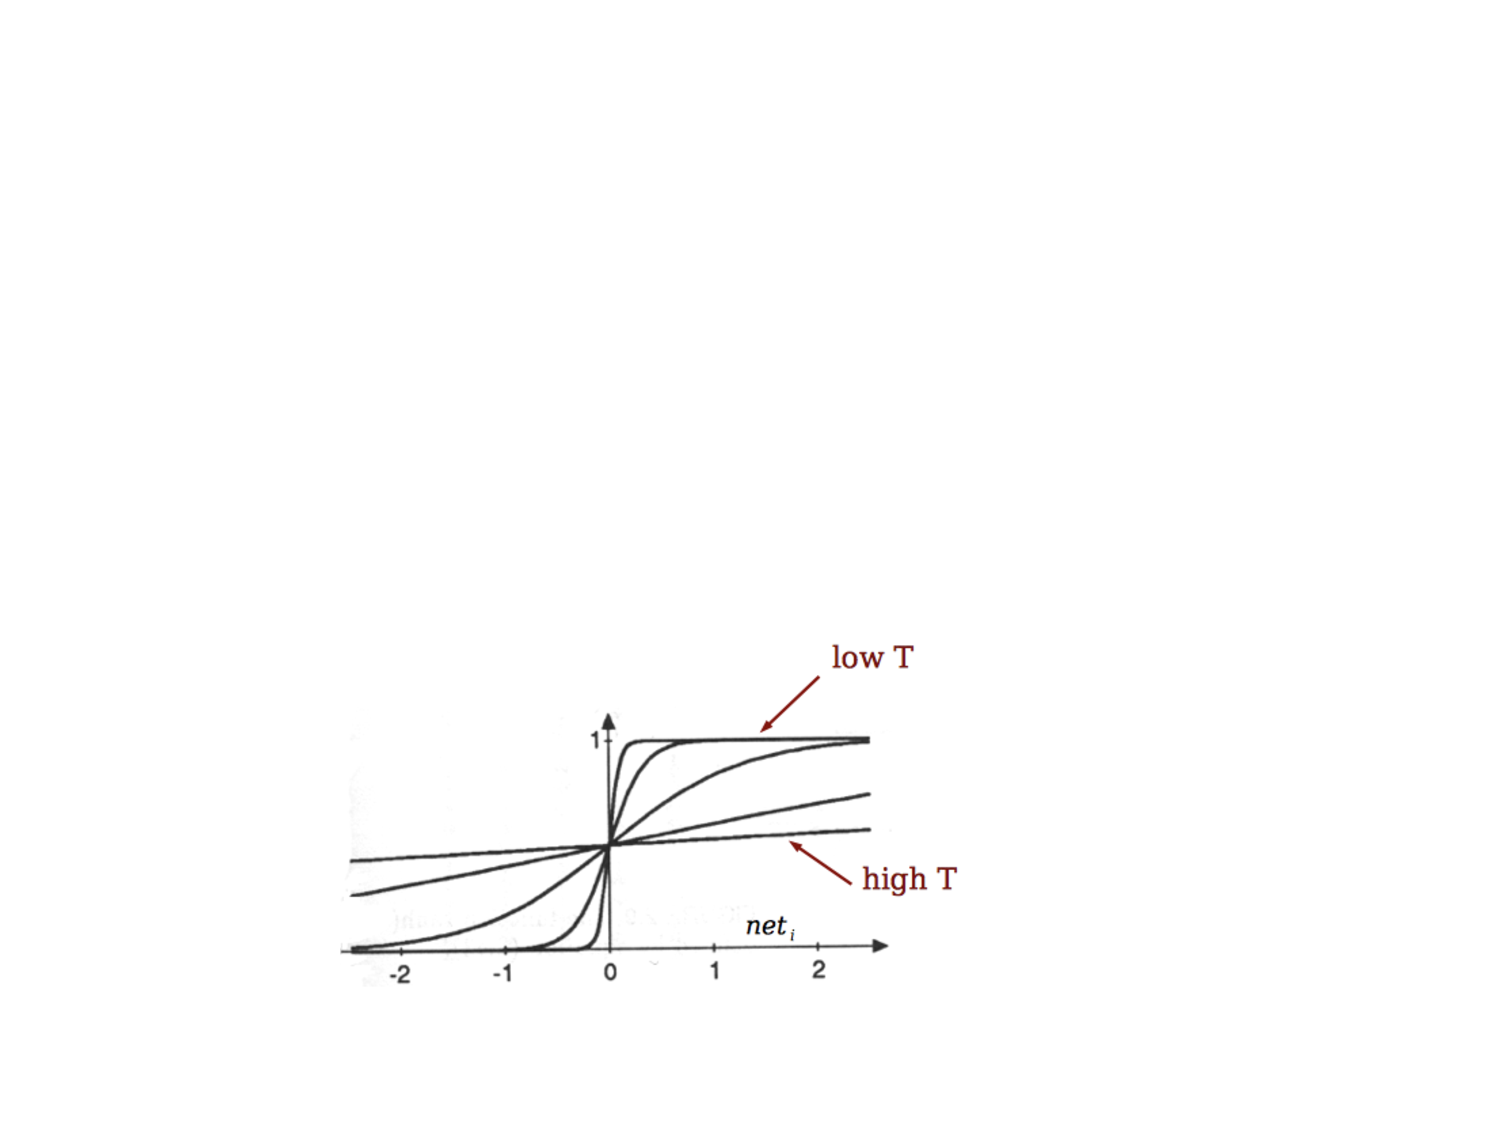
\includegraphics[width=0.7\linewidth]{figures/ch10_annealing.pdf}
	\caption{Logistische Funktion mit verschiedenen Temperaturparametern $T$.}
	\label{fig:ch10_annealing}
\end{figure}

Dieses ermöglicht das sogenannte \emph{simulated annealing}. Dabei wird mit einem großen Wert für $T$ begonnen, um anschließend durch langsames Verkleinern von $T$ ein \emph{Ausglühen} zu simulieren.
So erlaubt man dem Netz zu Beginn mehr Änderungen, was dazu führt, dass es eher aus lokalen Minima herausspringen kann.


% ------------------------------------------------------------------------
\subsection*{Lernregel}
\begin{hint}{Achtung!}{unvollstaendig-search-problem}
	Dieser Abschnitt ist nicht vollständig und muss überarbeitet werden.
\end{hint}
Neuronen einen Boltzmann-Maschine kann man in zwei Gruppen aufteilen:
\begin{enumerate}
	\item sichtbare Neuronen (\emph{visible units}) - Sie sind von außen sichtbar und können von dort Werte erhalten indem ihre Aktivierung, die mit der Ausgabe identisch ist, auf extern vorgegebene Werte $0$ oder $1$ gesetzt wird. 
	\item verdeckte Neuronen (\emph{hidden units}) - Sie sind von außen nicht einsehbar, werden jedoch vom Netzwerk benötigt, um die interne Repräsentation für komplexere Probleme zu bilden. 
\end{enumerate}

Eine beliebige Teilmenge sichtbarer Neuronen kann von außen mit Werten belegt werden. Jeder externe Eingabevektor, der an die sichtbaren Neuronen angelegt wird, wird so lange angelegt, bis sich die Boltzmann-Maschine im Temperaturgleichgewicht stabilisiert hat. Die Struktur der Umgebung kann dann als Wahrscheinlichkeitsverteilung aller $2^v$ Zustände der $v$ sichtbaren Neuronen betrachtet werden.

Ziel des Lernverfahrens der Boltzmann-Maschine ist es nun, die Gewichte des Netzes so anzupassen, dass es genau die gleiche Wahrscheinlichkeitsverteilung auf den sichtbaren Zuständen erreicht ($p(v_{\alpha})$), wie wenn man es im Temperaturgleichgewicht ohne externe Eingaben frei laufen lässt ($\tilde{p}(v_{\alpha})$).


% ------------------------------------------------------------------------
\subsection*{Search Problem}
\begin{hint}{Achtung!}{unvollstaendig-search-problem}
	Dieser Abschnitt ist nicht vollständig und muss überarbeitet werden.
\end{hint}

\begin{figure}[ht!] \centering 
	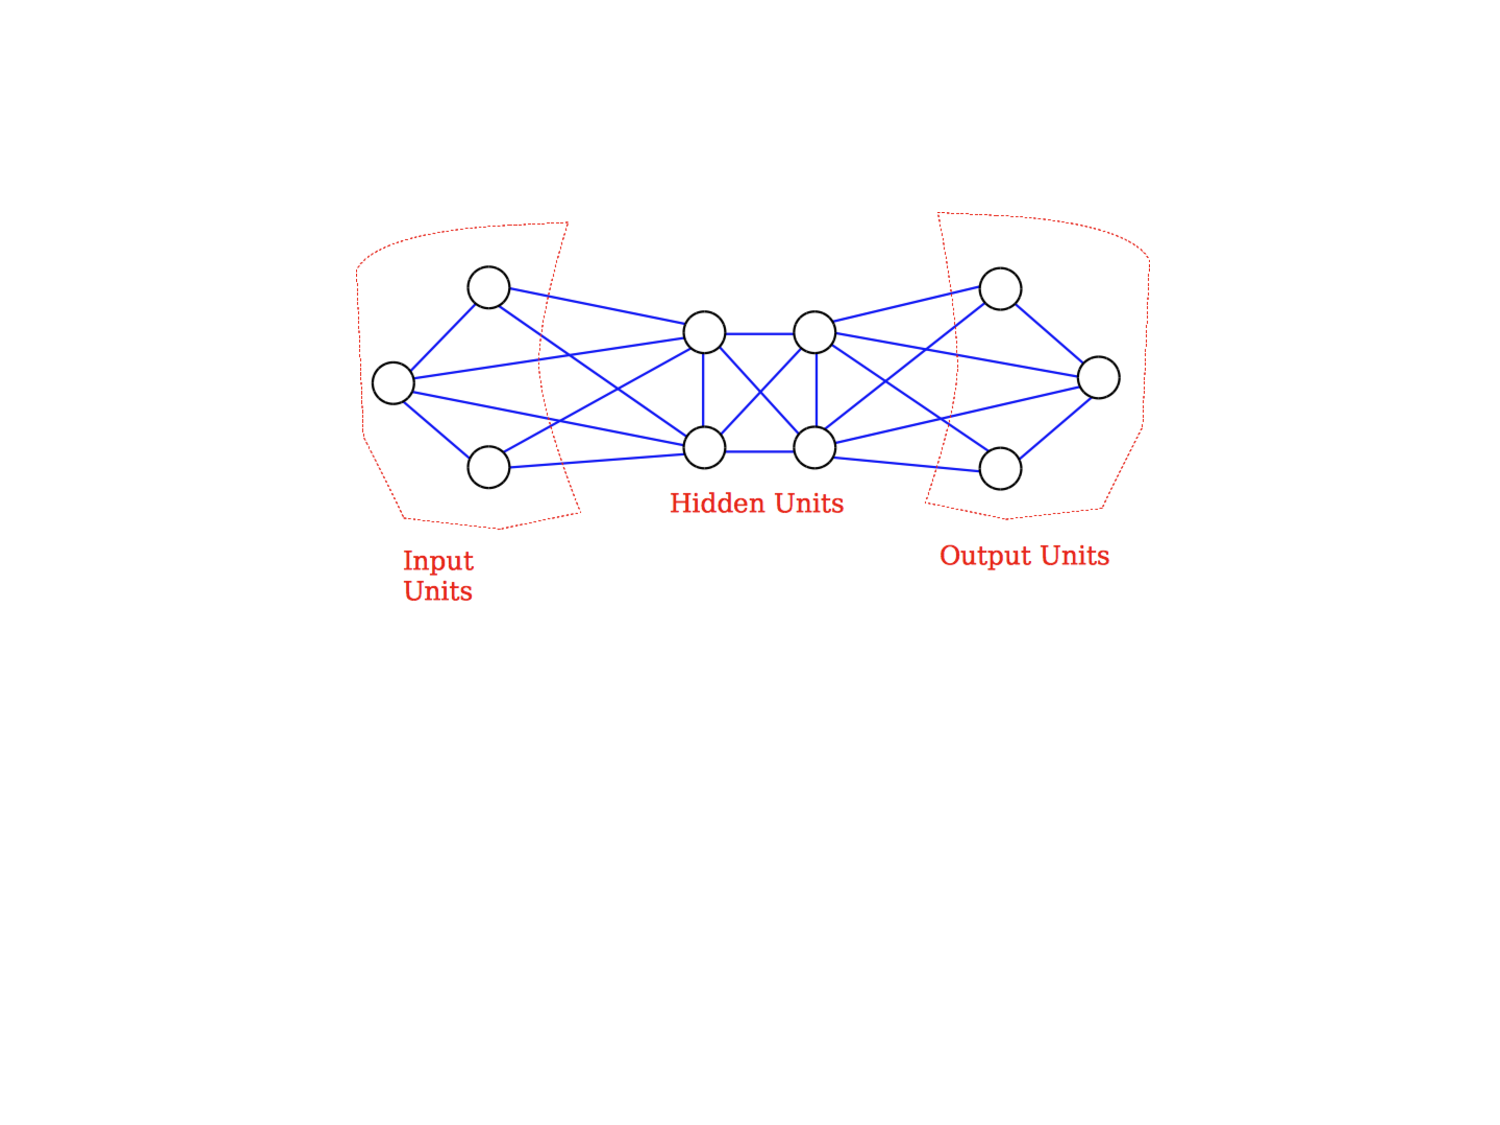
\includegraphics[width=\linewidth]{figures/ch10_boltzmann-search-problem.pdf}
	\caption{Boltzmann-Maschine mit Eingabe- und Ausgabeneuronen, sowie versteckten Neuronen.}
	\label{fig:ch10_boltzmann-search-problem}
\end{figure}



% ------------------------------------------------------------------------
\subsection*{Fazit}
Boltzmann-Maschinen mit ausreichend versteckten Neuronen können jede Funktion berechnen.

Das Training ist aufgrund der komplexen Struktur sehr langsam und rechenintensiv.




% ------------------------------------------------------------------------
% ------------------------------------------------------------------------
\subsection*{Restricted Boltzmann Machines (RBMs)}
\begin{hint}{Achtung!}{unvollstaendig-search-problem}
	Dieser Abschnitt ist nicht vollständig und muss überarbeitet werden.
\end{hint}
Restricted Boltzmann Machines sind die eingeschränkte Variante der Boltzmann-Maschinen. Es handelt sich um ein \emph{unüberwachtes} Lernverfahren, welches automatisch bedeutende Merkmale der Daten extrahiert.

Eine RBM muss dabei ein \emph{bipartiter Graph} sein, wie er in Abbildung \ref{fig:ch10_rbms-bipartiter-graph} dargestellt ist. RBMs bestehen damit aus zwei Schichten: Einer Schicht mit \emph{visible units} und eine mit \emph{hidden units}. 
Die Einschränkung der RBMs ist, dass es keine Kommunikation innerhalb einer Schicht gibt.
Der Vorteil der fehlenden Verbindungen zwischen den versteckten Knoten liegt im \emph{effizienteren} Training.

\begin{figure}[ht!] \centering 
	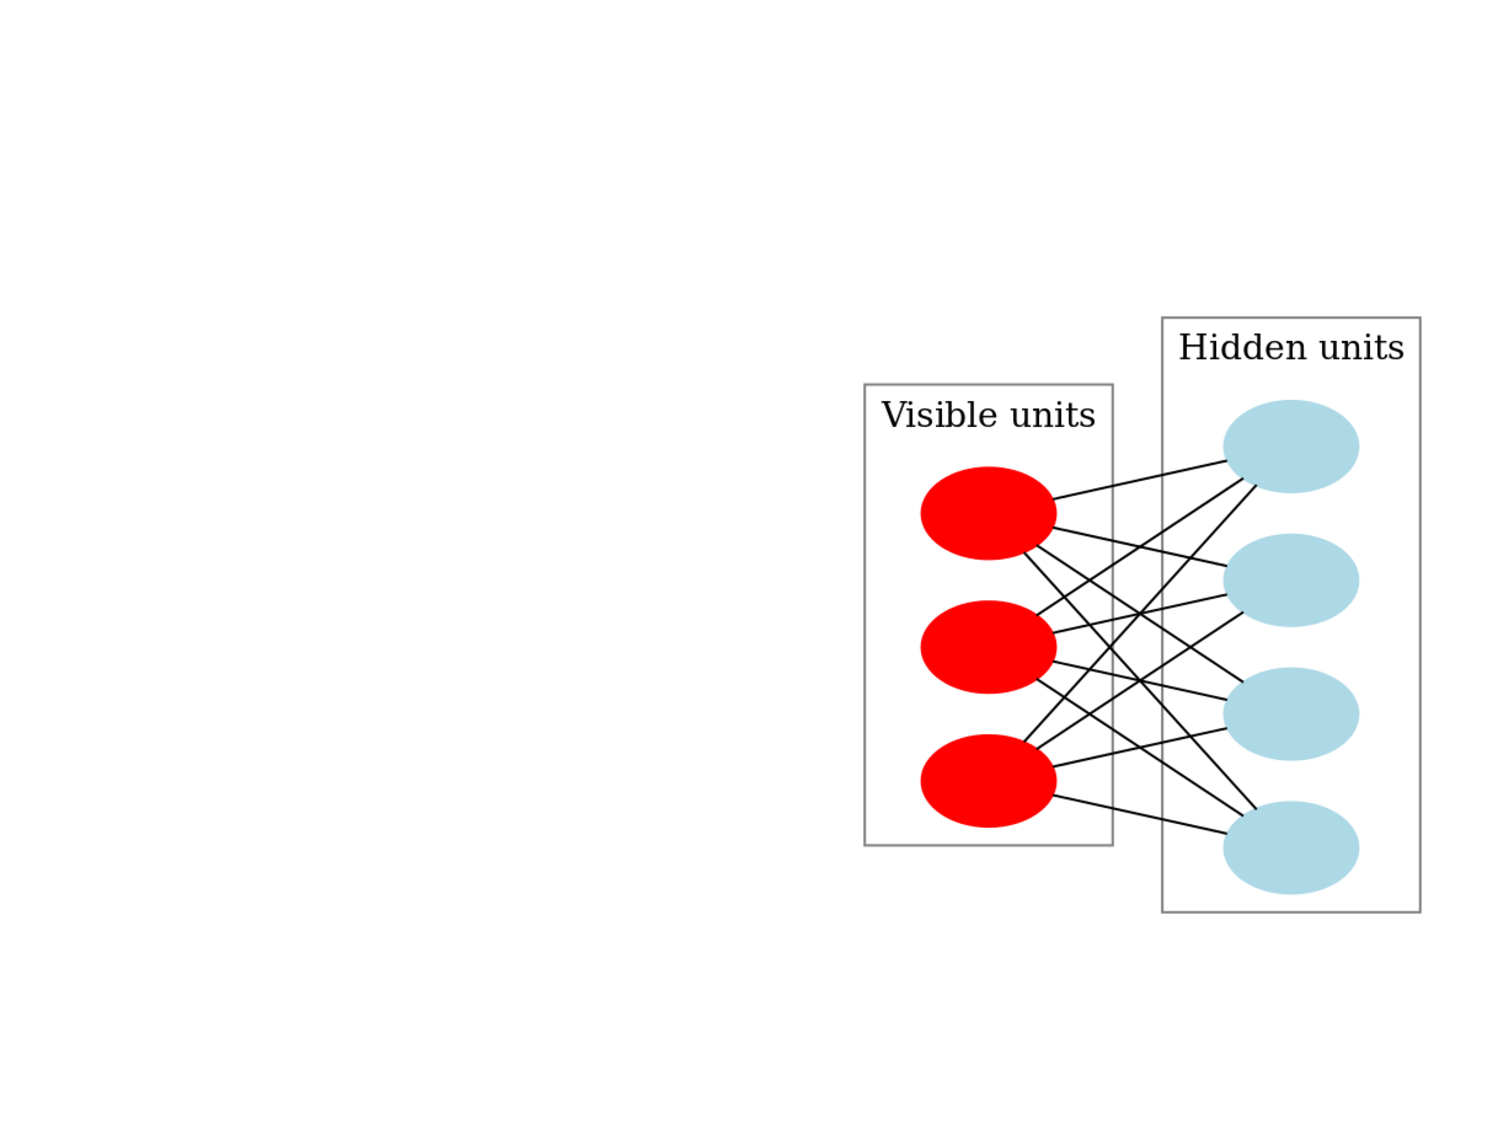
\includegraphics[width=0.5\linewidth]{figures/ch10_rbms-bipartiter-graph.pdf}
	\caption{Restricted Boltzmann-Maschine mit visible und hidden units.}
	\label{fig:ch10_rbms-bipartiter-graph}
\end{figure}

Die Energie $E$ ist definiert durch:
\[
	E(V,H) = - \sum_{i=1}^{m} \sum_{j=1}^{F} w_{ij} h_j v_i + 
		- \sum_{i=1}
\]
